%% Theorie.tex
%%
%\usepackage[ngerman]{babel}
%% ==============
\chapter{Algorithmen zur multivariaten Analyse}
\label{ch:algorithmen}
%% ==============

%{\bibliographystyle{babalpha-fl}}	% german style
{\bibliographystyle{babunsrt-fl}}

Multivariate Datenanalyse spielt in der experimentellen Teilchenphysik eine entscheidente Rolle, um die gro\ss en gemessenen Datenmengen untersuchen und auswerten zu k\"onnen. In diesem Kapitel werden zun\"achst einige Grundlagen der multivariaten Datenanalyse genannt, um sp\"ater genauer auf verschiedene Algorithmen und ihre Implementierungen einzugehen.

%% ===========================
\section{Grundlagen zur multivariaten Datenanalyse}
\label{ch:Theorie:sec:Algorithmen}
%% ===========================

Datenanalyse bezeichnet statistische Verfahren, mit deren Hilfe aus numerischen Daten Informationen gewonnen werden.
Bei multivariaten Analysemethoden (MVAs) werden mehrere Eingabegr\"o\ss en gleichzeitig statistisch untersucht. Dadurch ist eine Berechnung sehr aufw\"andig und somit manuell praktisch nicht zu bewerkstelligen. Mithilfe der zunehmenden Rechenleistung aktueller Computer ist dies jedoch m\"oglich und wird in vielen Bereichen immer wichtiger. Anwendungen finden MVAs beispielsweise im Finanzwesen, oder der Sprach-, Schrift- und Bilderkennung.\\
%Da die verwendeten Algorithmen die Eigenschaft haben anhand von bekannten Daten Vorhersagen f\"ur unbekannte Daten zu generieren, spricht man auch von maschinellem Lernen (machine learning).
%Die dazu verwendeten Algorithmen bezeichnet man auch als maschinelles Lernen (machine learning), da mit ihrer Hilfe versucht wird, die zugrunde liegenden Eigenschaften der Daten zu Lernen und Vorhersagen zu treffen.
Ziel ist es, mithilfe der Algorithmen aus bekannten Daten zu lernen und so Vorhersagen f\"ur unbekannte Daten zu generieren.
Man unterscheidet zwischen Regression, bei der eine kontinuierliche Ausgangsgr\"o\ss e gesucht wird, und Klassifikation, bei der eine diskrete Antwort gesucht wird \cite{SWB-455193959}.

Im Fall der \ttH-Analyse werden Regressionsmodelle verwendet, um physikalische Gr\"o\ss en wie beispielsweise die Higgs-Bosonmasse zu rekonstruieren. Bei der Klassifikation wird dagegen versucht, ein Ereignis einer Klasse zuzuordnen, also entweder Signal oder Untergrund. Im Folgenden werden ausschlie\ss lich Klassifikationsprobleme behandelt.

Die St\"utzvektormethode (support vector machine), Random Forest und Neuronale Netze sind Beispiele f\"ur Methoden zur Klassifikation. 
%Es existieren verschiedene Ans\"atze zur Klassifikation. Beispiele sind die St\"utzvektormethode, wobei jedoch die englische Bezeichnung support vector machine (SVM) gebr\"auchlich ist, Random Forest (RF), was zuf\"alliger Wald bedeutet und mehrere zuf\"allig erstellte Entscheidungsb\"aume (Abschnitt \ref{ch:Algorithmen:subsec:Entscheidungsbaum}) bezeichnet, oder Neuronale Netze. 
Ein weiteres Beispiel sind verst\"arkte Entscheidungsb\"aume (Boosted Decision Trees (BDTs)). Da hiervon verschiedene Implementationen im Kapitel \ref{ch:vergleich} untersucht und getestet werden sollen, werden sie im folgenden Abschnitt \ref{ch:Algorithmen:sec:BDT} genauer beschrieben.

%% ===========================
\section{Verst\"arkte Entscheidungsb\"aume}
\label{ch:Algorithmen:sec:BDT}
%% ===========================

Verst\"arkte Entscheidungsb\"aume (Boosted Decision Trees, BDTs) sind eine h\"aufig genutze Methode der multivariaten Datenanalyse. Im Folgenden werden sie anhand eines Beispiels erkl\"art. Bei diesem handelt es sich um zwei zweidimensionale Gau\ss verteilungen die sich \"uberlappen. Eine stellt das Signal dar, die andere dient als Untergrund. Der Erwartungswert der Signalverteilung ist bei $\mu_X=\mu_Y=0$, der der Untergrundverteilung bei $\mu_X=\mu_Y=1$. Beide haben eine Standardabweichung von $\sigma=1$. In Abbildung \ref{fig:2dgauss_scat} ist ein Streudiagramm mit Trainings-Datenpunkten dargestellt. Insgesamt haben sowohl Signal als auch Untergrund 10001 Ereignisse, zur besseren \"Ubersicht sind allerdings nur jeweils 1000 dargestellt.\\
Die folgenden Abschnitte sind gr\"o\ss tenteils an \cite{SWB-307748006} angelehnt.

\begin{figure}[tbp]
 \begin{center}
   \includegraphics[width=\textwidth]{graphics/2d_scatter.pdf}
   \parbox[b]{12cm}{
     \caption[Streudiagramm mit Trainings-Datenpunkten]
             {\label{fig:2dgauss_scat}Ein Streudiagramm mit je 1000 Signal- und Untergrundereignissen. Signalereignisse sind rot, Untergrundereignisse blau dargestellt.}
   }
 \end{center}
\end{figure}

%% ===========================
\subsection{Entscheidungsb\"aume}
\label{ch:Algorithmen:subsec:Entscheidungsbaum}
%% ===========================

Entscheidungsb\"aume (Decision Trees) unterteilen den Bereich der zu klassifizierenden Objekte anhand gerader Schnitte auf dessen Eigenschaften (Variablen) in mehrere Sequenzen. Wieviele dieser Sequenzen ab dem Wurzelknoten erstellt werden, wird durch die Tiefe (depth) des Baumes angegeben. Man unterscheidet zwischen zwei Arten, bin\"aren B\"aumen mit diskreten R\"uckgabewerten zur Unterscheidung mehrerer Klassen (classification trees), zum Beispiel Signal und Untergrund sowie denjenigen mit kontinuierlicher Antwort (regression trees) \cite{SWB-455193959}. Eine h\"aufige Implementierung von Entscheidungsb\"aumen ist CART (classification and regression trees). Auf diese Weise implementierte B\"aume eignen sich sowohl f\"ur Klassifikationen als auch f\"ur Regressionen \cite{CART}.\\
In Abbildung \ref{fig:DecicionTree} ist ein Beispiel eines Baumes mit der Tiefe zwei zu sehen. An jedem Knoten werden die Objekte aufgrund ihrer Eigenschaften und Kriterien in Signal und Untergrund unterteilt. Im Wurzelknoten ist der erste diskriminierende Schnitt angegeben. Alle Objekte mit einem Y-Wert gr\"o\ss er als \num{0,4} werden als untergrundartig eingestuft. In der n\"achsten Stufe des Baumes werden f\"ur jede der beiden zuvor getrennten Mengen Schnitte auf den X-Wert angewendet. In Abbildung \ref{fig:depht2} ist die Ausgabe (output) dieses Baumes abgebildet. Das hei\ss t, jedem Punkt wird entsprechend seiner X- und Y-Koordinaten ein Wert zugeordnet, der angibt, ob der Punkt eher als Signal oder als Untergrund klassifiziert wurde. H\"ohere Werte werden f\"ur signalartige Punkte verwendet, niedrigere f\"ur untergrundartige. Es sind die verschiedenen Schnitte des Baumes zu erkennen.\\
%\begin{figure}[tbp]
% \begin{center}
%  \begin{minipage}[b]{0.5\textwidth}  
%   \includegraphics[width=\textwidth]{graphics/tree.pdf}
%   \centering (a)
%  \end{minipage}%
%  \begin{minipage}[b]{0.5\textwidth}
%   \includegraphics[width=\textwidth]{graphics/tree_depht2.pdf}
%   \centering (b)
%  \end{minipage}
%   \parbox[b]{12cm}{
%     \caption[Entscheidungsbaumes der Tiefe 2]
%             {\label{fig:DecicionTree} \it schematische Abbildung eines Entscheidungsbaumes der Tiefe 2. X und Y sind die Variablen anhand denen durch cuts (Zahlen nach den Variablen) zwischen Untergrund und Signal unterschieden werden soll.\\Erstellt mit TMVA}
%   }
% \end{center}
%\end{figure}

\begin{figure}[tbp]
\centering     %%% not \center
\subfigure[Entscheidungsbaum der Tiefe zwei]{\label{fig:DecicionTree}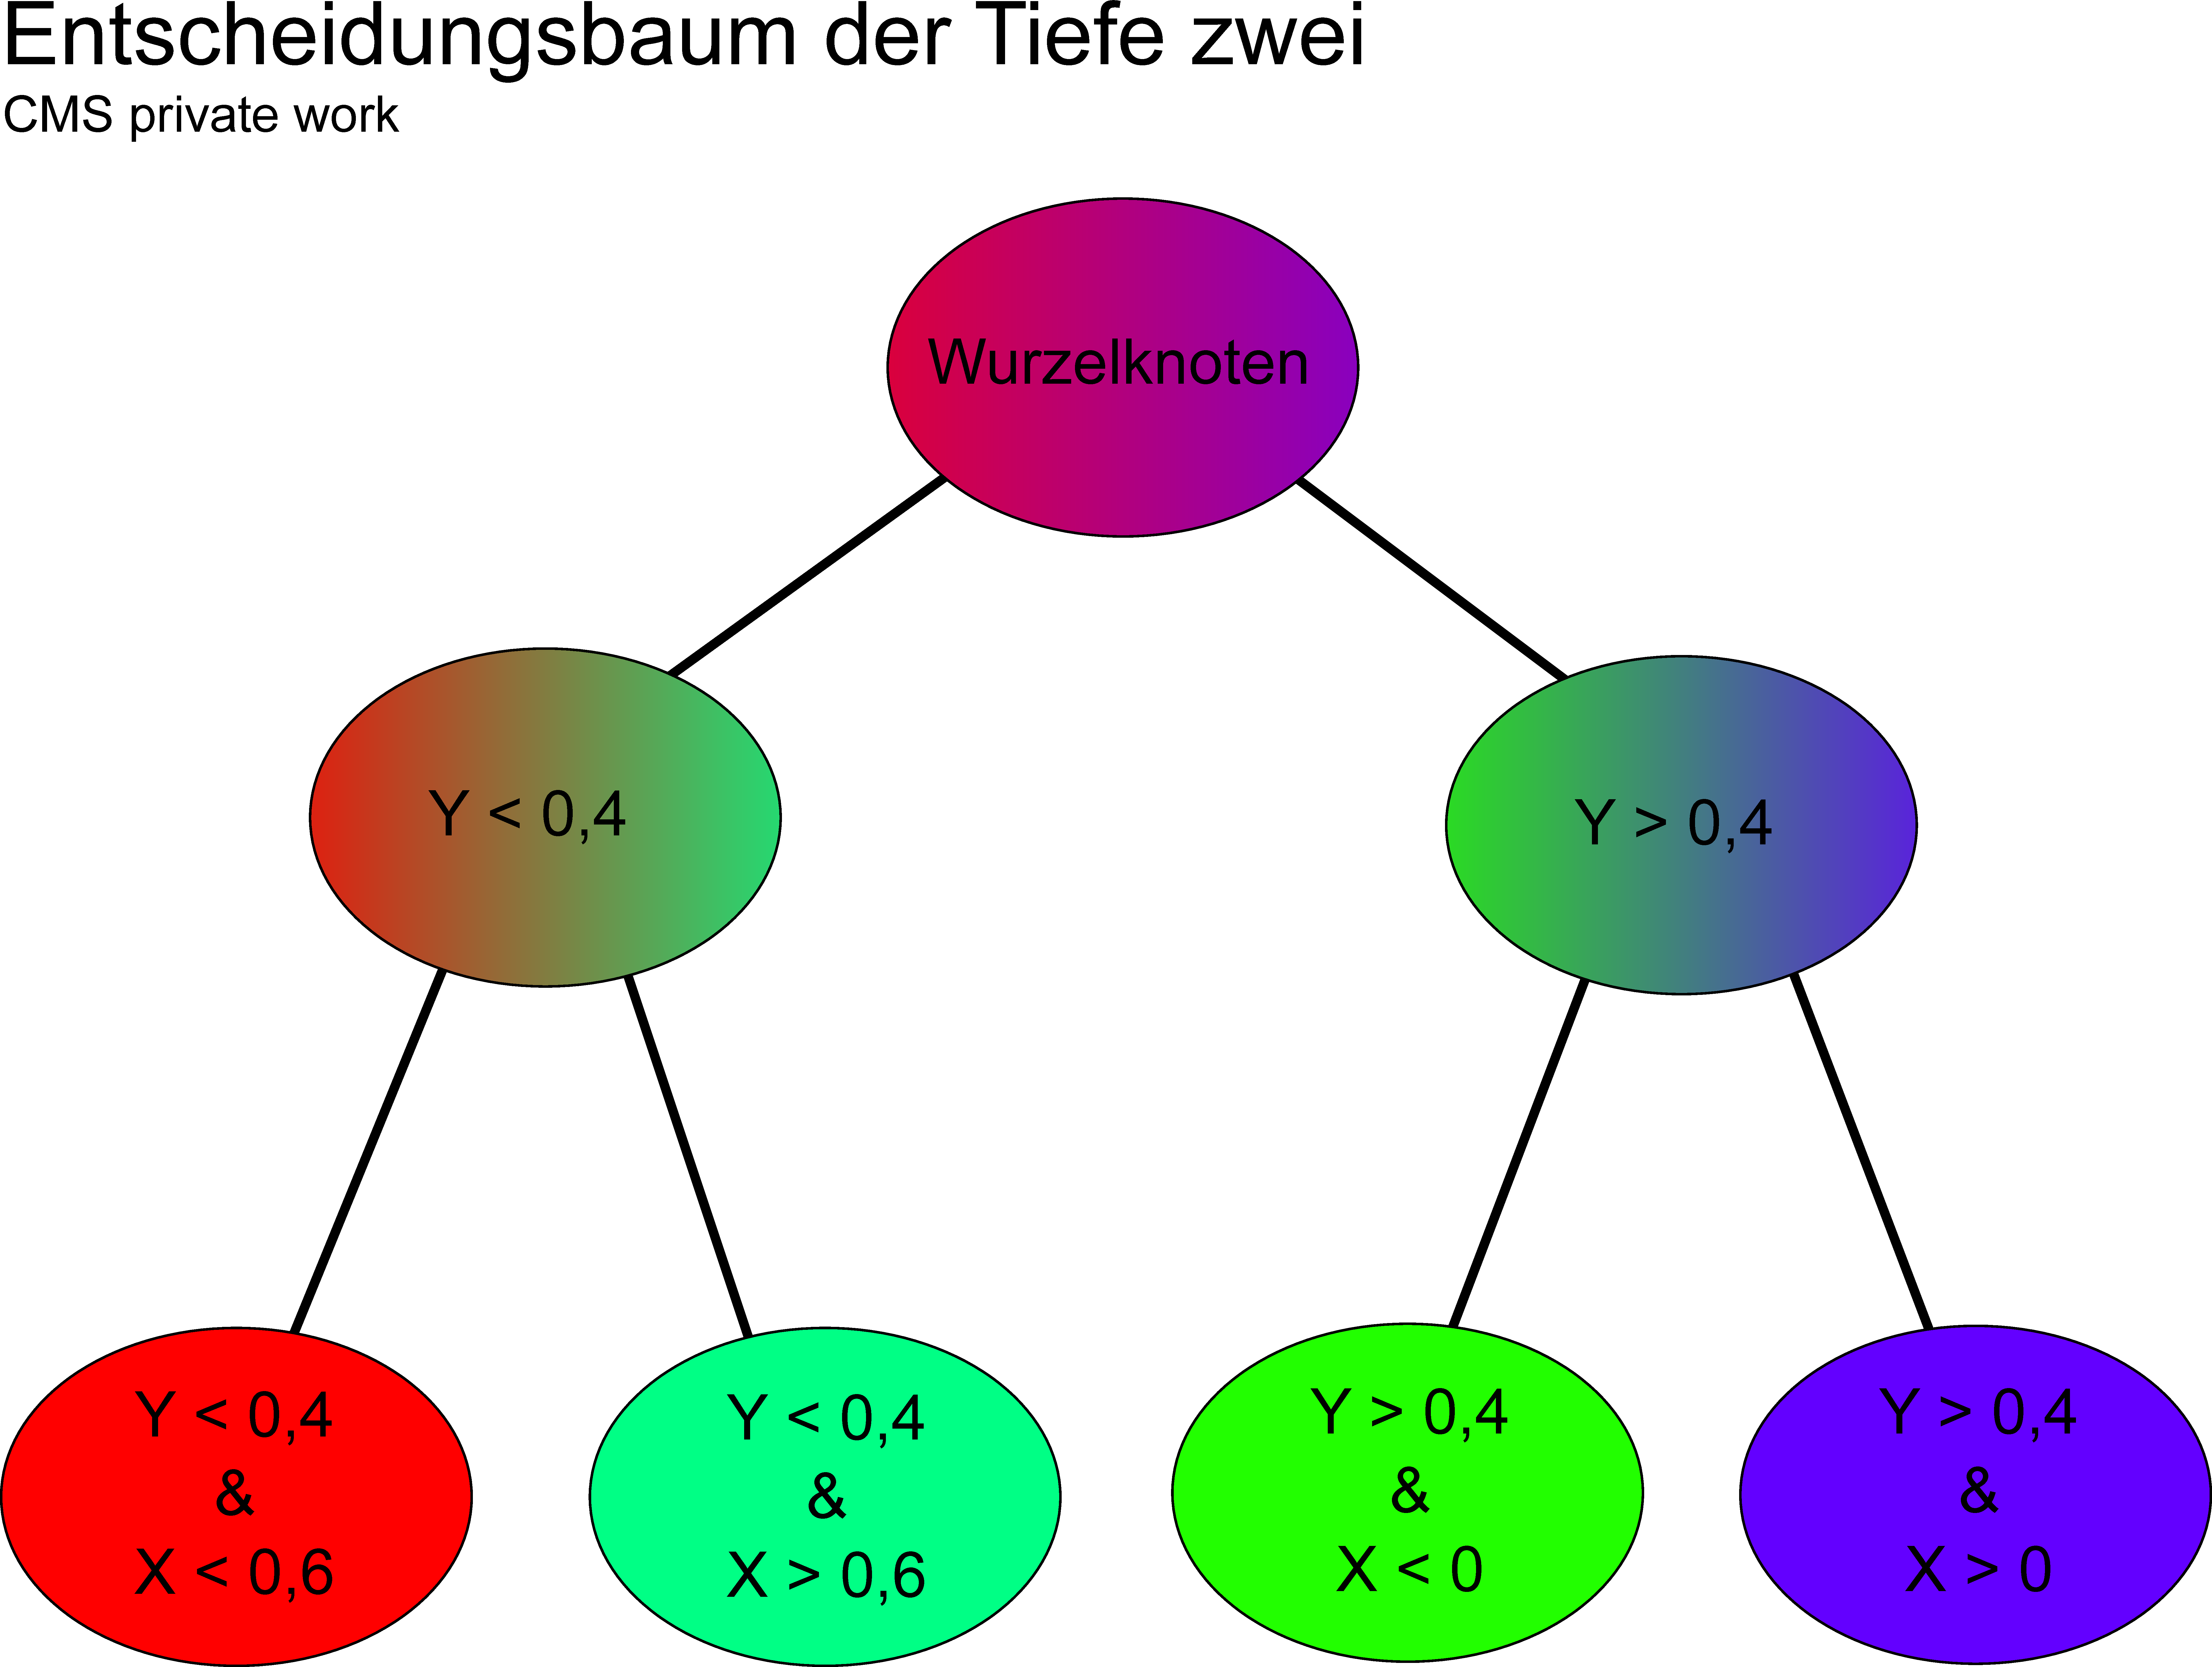
\includegraphics[width=0.7\textwidth]{graphics/tree_d22.pdf}}
\subfigure[Klassifizierung des Baumes]{\label{fig:depht2}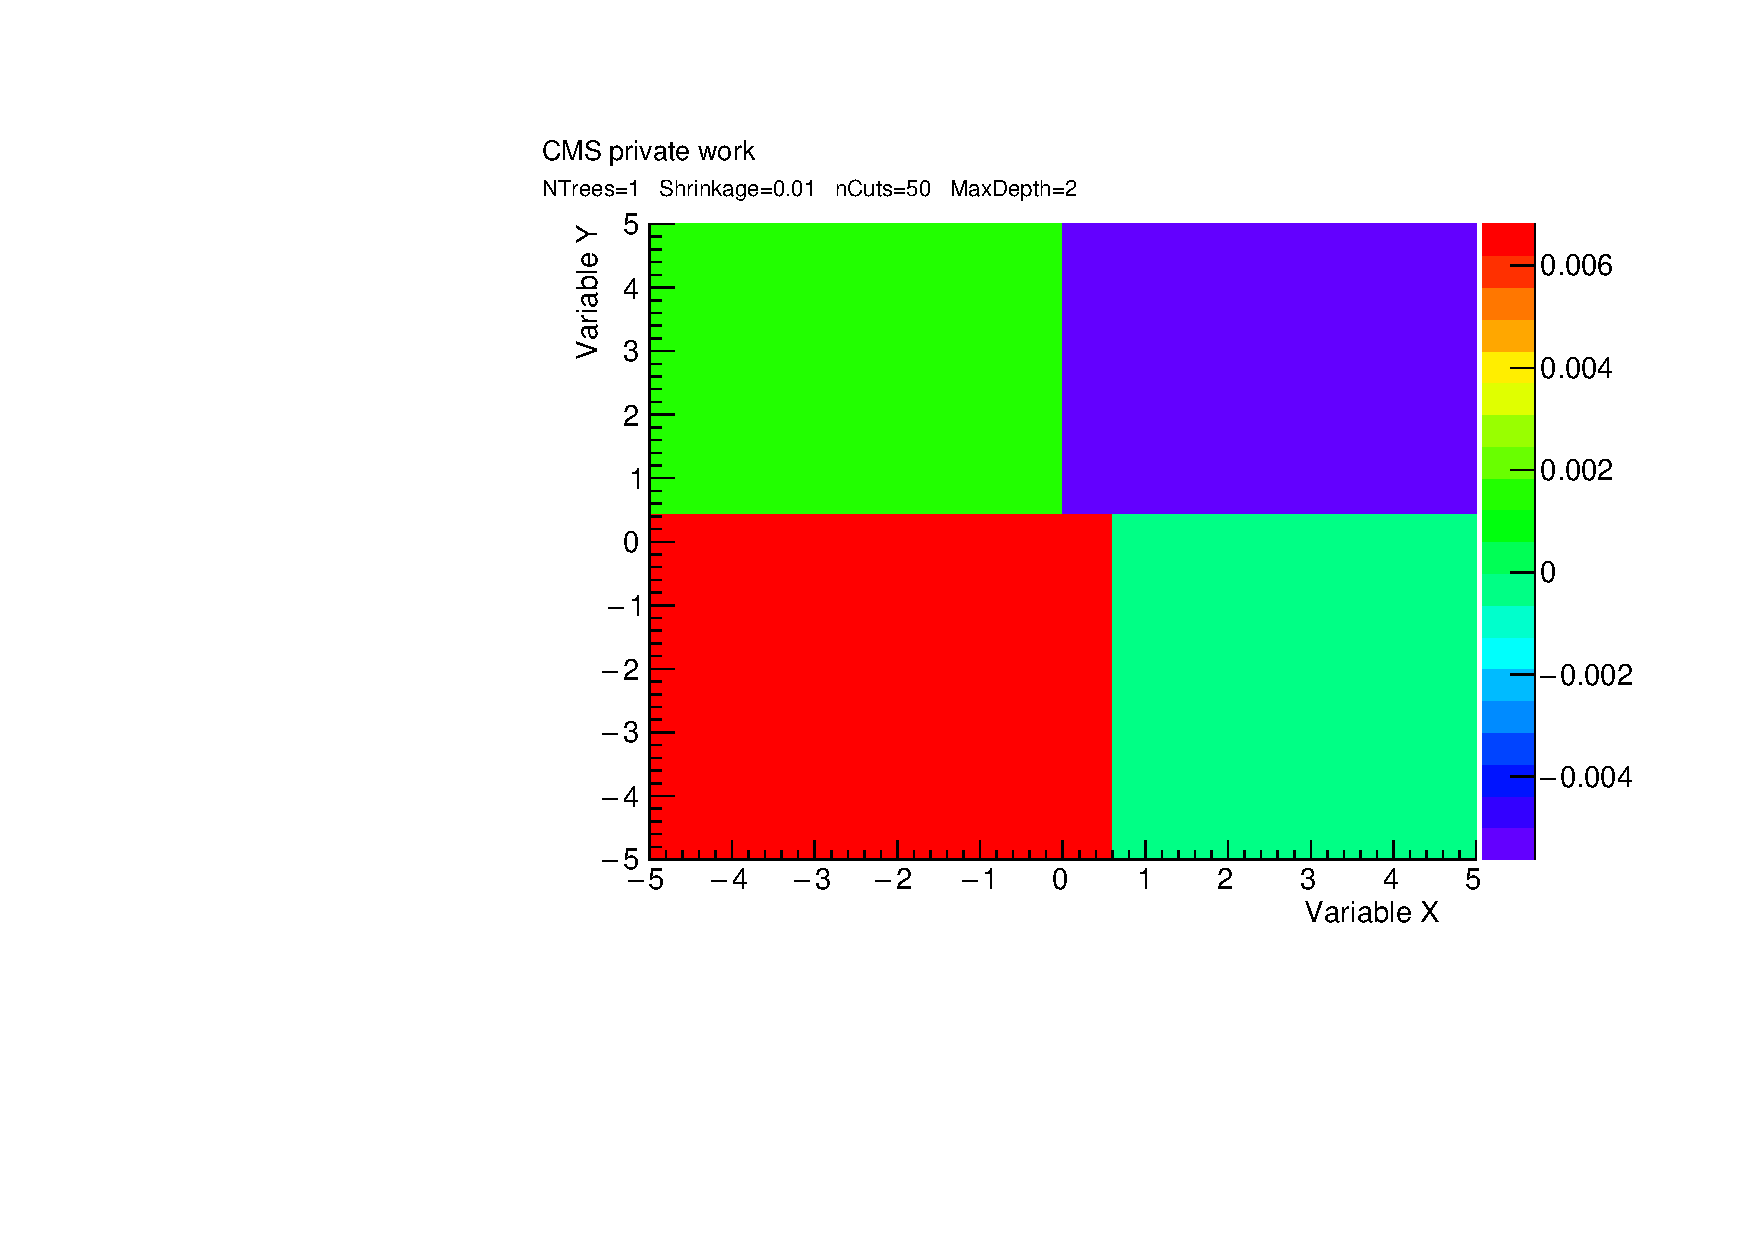
\includegraphics[width=0.85\textwidth]{graphics/tree_depht2_1.pdf}}
\parbox[b]{12cm}{
\caption{Oben ist eine schematische Abbildung eines Entscheidungsbaumes der Tiefe 2 abgebildet. X und Y sind die Variablen, anhand derer durch Schnitte (Zahlen nach den Variablen) zwischen Untergrund und Signal unterschieden werden soll. Die untere Graphik zeigt die Klassifikation, die mithilfe des Baumes erstellt wurde. Gr\"o\ss ere Ausgabewerte sind rot gef\"arbt und stehen f\"ur signalartige Ereignisse, kleinere blau und stehen f\"ur untergrundartige Ereignisse.}
}
\end{figure}

Die Trennung ist allerdings noch sehr grob, selbst wenn man die Tiefe des Baumes deutlich erh\"oht, wie in Abbildung \ref{fig:tree_depht100} mit der Tiefe 100 zu sehen, wird diese nicht deutlich besser. Eine Verbesserung ist beispielsweise m\"oglich, indem man mehrere Entscheidungsb\"aume so miteinander verkn\"upft, dass sie zusammen eine starke Klassifikation erm\"oglichen. Eine dieser Methoden ist das Verst\"arken von Entscheidungsb\"aumen (Boosting).




%BDTs vereinen durch Boosting und Bagging (aus dem Englischen von bootstrap aggregation abgeleitet) mehrere Entscheidungsb\"aume zu einem starken Kla\ss ifikator.

%% ===========================
\subsection{Verst\"arken von Entscheidungsb\"aumen}
\label{ch:Algorithmen:subsec:Boosting}
%% ===========================

Durch das Verst\"arken von Entscheidungsb\"aumen (Boosting) soll die G\"ute der Gesamtklassifikation gegen\"uber der eines einzelnen Baumes erh\"oht werden. Dazu werden mehrere B\"aume hintereinander trainiert. Damit diese sich voneinander unterscheiden, werden bei nachfolgenden B\"aumen die falsch klassifizierten Ereignisse anders behandelt\\
Die einfachste Methode ist, das Gewicht jedes falsch klassifizierten Ereignisses auf die gleiche Weise anzupassen. Eine weitere Verbesserung l\"asst sich erzielen, indem man eine Ausgleichsfunktion (loss function) einf\"uhrt. Diese ordnet jedem Ereignis ausgehend von der aktuellen BDT-Ausgabe einen Wert zu, der bei richtiger Klassifikation minimal ist. Dadurch ist es m\"oglich, die Gewichte so anzupassen, dass die Ausgleichsfunktion minimiert wird.\\
Wenn die zu trennenden Klassen mit $y=\pm1$ bezeichnet werden und $f(x)$ die Vorhersage des BDTs f\"ur das Ereignis $x$ ist, also $sign(f)$ die jeweilige Klasse vorhersagt, so kann man die einfache Methode der Neugewichtung mathematisch mit
\beq
L = I(sign(f(x))\neq y)
\label{eq:missclass_loss}
\eeq
beschreiben. Dabei nimmt die Funktion I den Wert $1$ an, wenn die Vorhersage nicht der wahren Klasse $y$ entspricht oder $0$, wenn die vorhergesagte mit der wahren Klasse \"ubereinstimmt.\\
Eine etwas komplexere Ausgleichsfunktion ber\"ucksichtigt die quadratischen Fehler der BDT-Vorhersage
\beq
L = (y-f(x))^2.
\label{eq:squarederror_loss}
\eeq
Diese Funktion bildet eine Parabel um den wahren Wert. Je weiter die Vorhersage davon abweicht, desto h\"oher wird das Ereignis gewichtet. Nachteilig ist dabei, dass positive wie negative Differenzen gleich stark korrigiert werden. So werden beispielsweise f\"ur $y=1$ BDT-Ausgaben von $f=0$ und $f=2$ gleich stark korrigiert, obwohl $f=0$ gar keine Klassifikation zul\"asst, w\"ahrend $f=2$ deutlich auf $y=1$ hinweist. Daher verwendet man meist Funktionen, die negative Abweichungen st\"arker umgewichten, wie beispielsweise die exponentielle Ausgleichsfunktion
\beq
L = \exp(-y\cdot f(x)).
\label{eq:exp_loss}
\eeq
Diese Ausgleichsfunktion wird beispielsweise von AdaBoost (kurz f\"ur Adaptive Boosting) \cite{ADABoost}, dem ersten entwickelten Boosting-Algorithmus, verwendet. Problematisch an der exponentiellen Ausgleichsfunktion ist, dass sie nicht besonders robust gegen\"uber Ausrei\ss ern ist.\\
Dieses Problem behebt der Gradient-Boosting-Algorithmus \cite{Friedman00greedyfunction}. Dabei wird eine zus\"atzliche Ausgleichsfunktion $L$ definiert, die nicht mithilfe der \"ublichen Vorgehensweise minimiert werden kann, sondern \"uber einen Ansatz der steilsten Abnahme (steepest-descent) minimiert werden muss. Dazu wird zun\"achst der negative Gradient der Ausgleichsfunktion gebildet:
\beq
r_m=\left|\frac{\partial L(y,f(x))}{\partial f(x)}\right|_{f=f_{m-1}}.
\label{eq:pseudo_residual}
\eeq
Die $r_m$ nennt man auch Pseudo-Residuen. Hierbei bezeichnet $m$ die jeweilige Boosting-Iteration. Danach wird ein zus\"atzlicher Regressionsbaum trainiert, f\"ur den als Zielwerte die Pseudo-Residuen anstatt der Klassen $y$ verwendet werden \cite{Hocker:2007ht}.\\
Die Endknoten des Regressionsbaums bezeichnet man mit $R_{jm}$, wobei $j$ den jeweiligen Knoten und $m$ den aktuellen Klassifikationsbaum numeriert. Insgesamt erh\"alt man eine BDT-Ausgabe von
\beq
\hat f(x) = f_M(x),
\eeq
wobei jede Iteration wie
\beq
f_m(x) = f_{m-1}+\nu\cdot\sum_{j=1}^J\gamma_{jm}I(x \in R_{jm})
\eeq
berechnet wird.\\
Dabei ist $\gamma_{jm}$ die Stelle, an der die Ausgleichsfunktion minimal wird. Die Funktion $I$ nimmt die Werte $1$ oder $0$ an, je nachdem ob das Ereignis $x$ im entsprechenden Endknoten des Regressionsbaumes liegt oder nicht. Die Gesamtanzahl der trainierten B\"aume ist $M$.
Der Parameter $\nu$ ist die Lernrate (shrinkage oder learning rate), der Werte von Null bis Eins annehmen kann. Mit diesem Parameter kann die Boosting Prozedur kontrolliert werden. Je kleiner der Wert ist, desto geringer werden die neu trainierten B\"aume gewichtet. Somit kann einem Erlernen von statistischen Fluktuationen entgegengewirkt werden (siehe auch Abschnitt \ref{ch:Algorithmen:subsec:overtraining}). Bei kleiner Lernrate sollte die Anzahl an B\"aumen h\"oher gew\"ahlt werden als bei gr\"o\ss erer. Die Bezeichnungen dieser und weiterer Optionen mit kurzer Erkl\"arung sind in Abschnitt \ref{ch:Vergleich:sec:Vergleichbarkeit} beschrieben.

In Abbildung \ref{fig:boosting} sind zum Vergleich die R\"uckgabewerte von einem einzelnen Entscheidungsbaum der Tiefe 100 (Abbildung \ref{fig:tree_depht100}) sowie diejenigen von BDTs der Tiefe zwei mit zwei (Abbildung \ref{fig:BDT_nTree2}), zehn (Abbildung \ref{fig:BDT_nTree10}) und hundert (Abbildung \ref{fig:BDT_nTree100}) Boosting-Schritten gezeigt. Alle diese Klassifikationen wurden mit dem Gradient-Boosting-Algorithmus von TMVA (siehe Abschnitt \ref{ch:Algorithmen:subsec:TMVA}) erstellt. Man erkennt, dass bei diesem einfachen Beispiel die Ausgabe der BDTs schon ab zehn Einzelb\"aumen deutlich glatter wird und sie so eine st\"arkere Unterscheidung erm\"oglichen.

\begin{figure}[tbp]
\centering     %%% not \center
\subfigure[Klassifikation eines Baumes der Tiefe 100]{\label{fig:tree_depht100}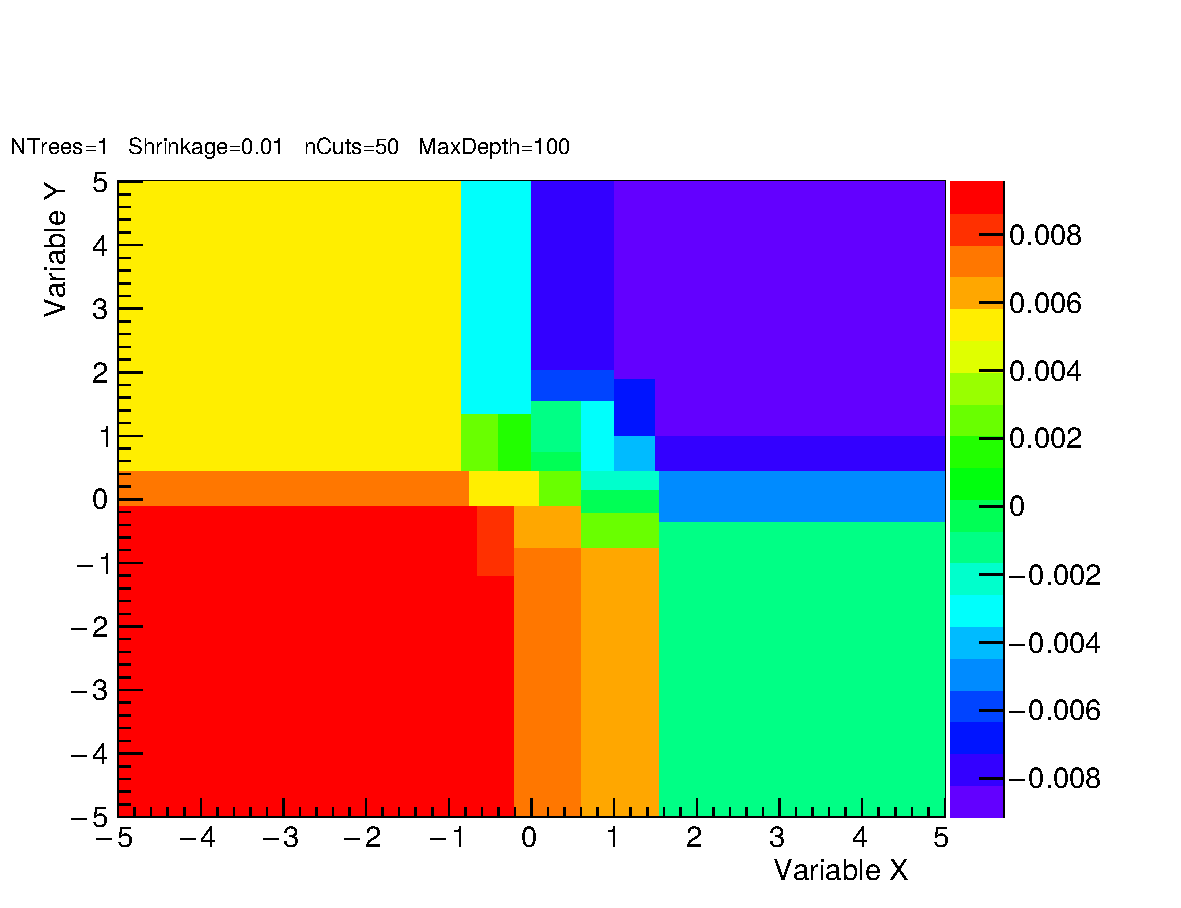
\includegraphics[width=0.85\textwidth]{graphics/tree_depht100.pdf}}
\subfigure[BDT Klassifikation mit 2 Trees]{\label{fig:BDT_nTree2}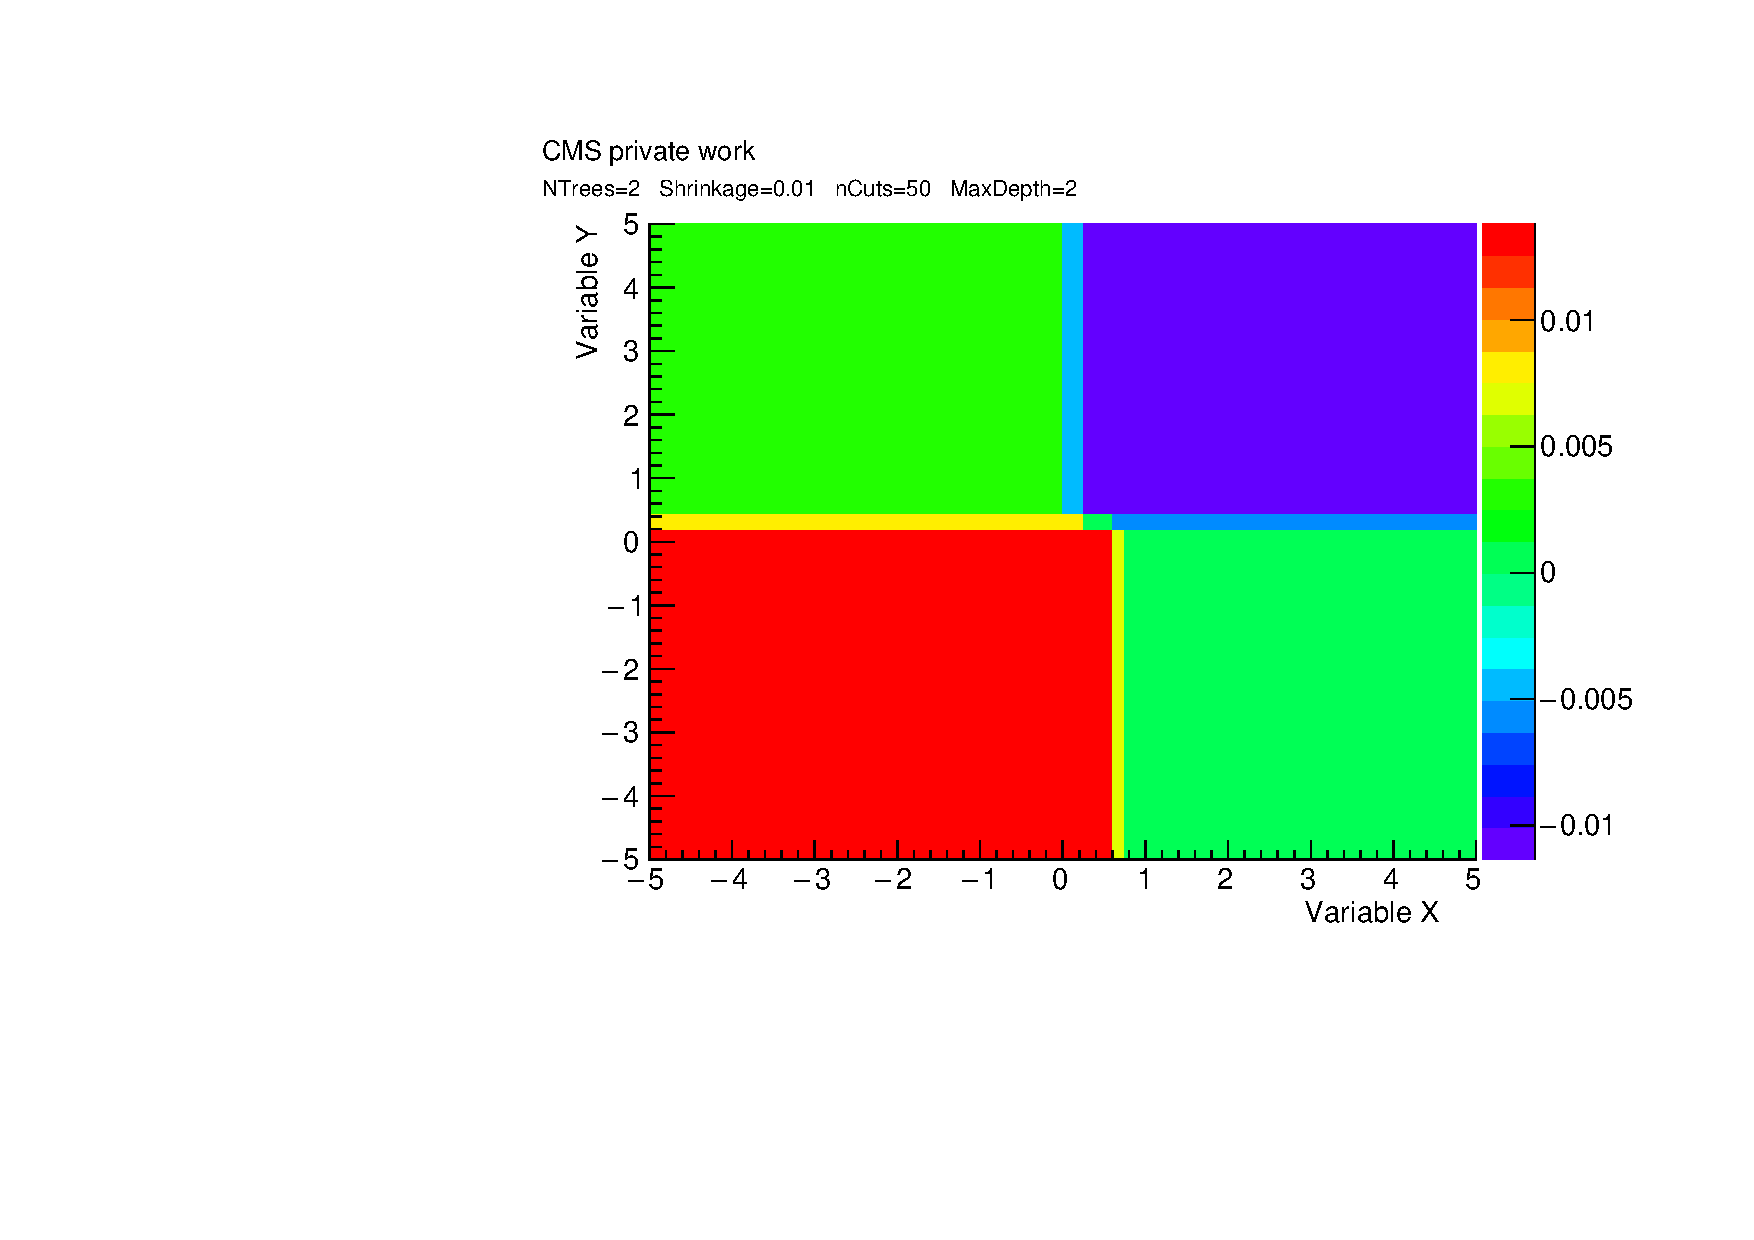
\includegraphics[width=0.85\textwidth]{graphics/tree_depht2_2.pdf}}
\parbox[b]{12cm}{
\caption{Die obere Grafik zeigt die Klassifikation, die mit einem einzelnen Entscheidungsbaum der Tiefe 100 erreicht wird. Signalartige Regionen sind mit positiver Ausgabe in Rott\"onen dargestellt, untergrundartige ergeben eine negative Ausgabe und sind in Blaut\"onen dargestellt. In der unteren Abbildung ist die Klassifikation eines BDT mit zwei B\"aumen der Tiefe zwei zu sehen.}
}
\label{fig:boosting}
\end{figure}

\begin{figure}[tbp]
\centering     %%% not \center
\subfigure[BDT Klassifikation mit 10 Trees]{\label{fig:BDT_nTree10}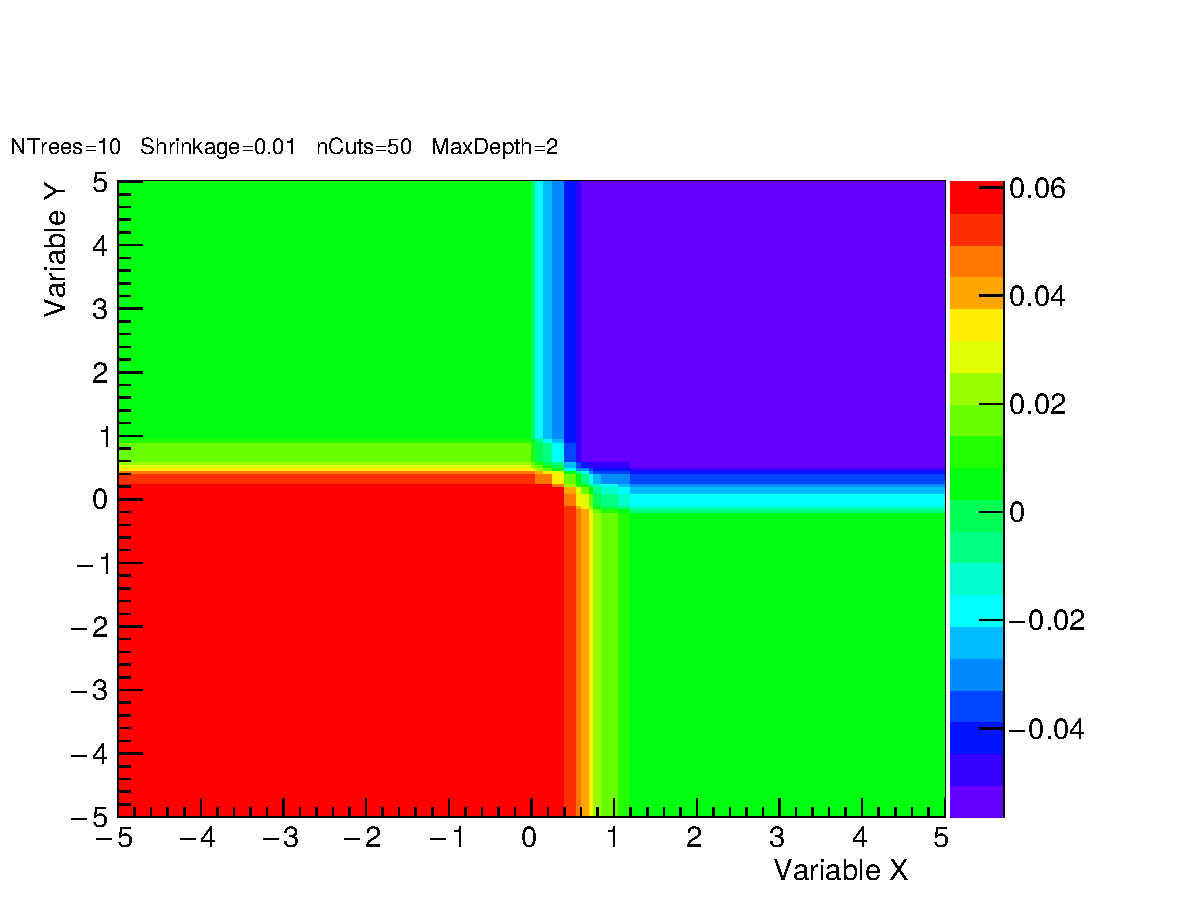
\includegraphics[width=0.85\textwidth]{graphics/tree_depht2_3.pdf}}
\subfigure[BDT Klassifikation mit 100 Trees]{\label{fig:BDT_nTree100}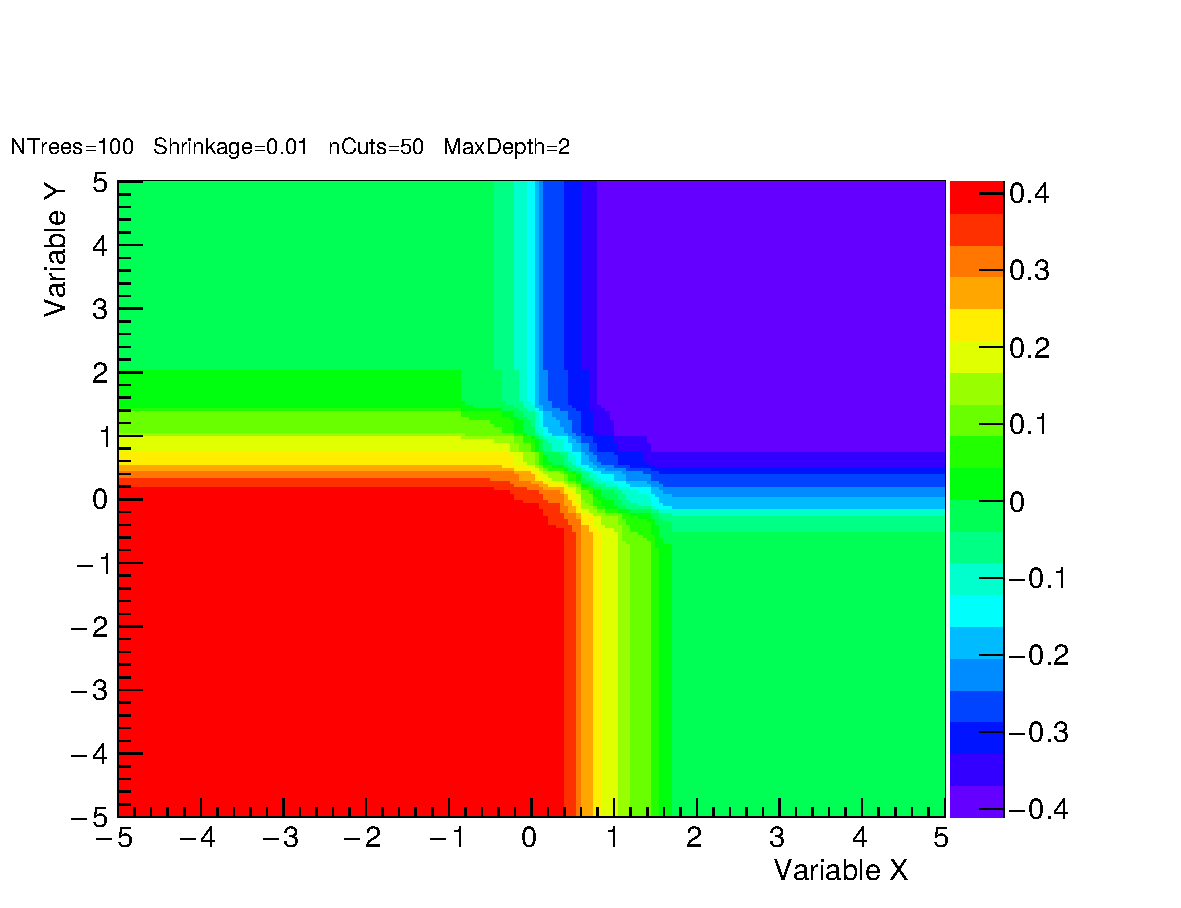
\includegraphics[width=0.85\textwidth]{graphics/tree_depht2_4.pdf}}
\parbox[b]{12cm}{
\caption{Oben ist die Klassifikation eines BDT mit zehn B\"aumen der Tiefe zwei, unten die eines BDT mit 100 B\"aumen der Tiefe zwei abgebildet. Signalartige Regionen sind mit positiver Ausgabe in Rott\"onen dargestellt, untergrundartige ergeben eine negative Ausgabe und sind in Blaut\"onen dargestellt.}
}
\label{fig:boosting}
\end{figure}

%% ===========================
%\subsection{Variieren der Trainingsereignisse (Bagging)}
%\label{ch:Algorithmen:subsec:Bagging}
%% ===========================

%Bagging (aus dem Englischen von bootstrap aggregation abgeleitet) bezeichnet eine Technik die Trainingsereignisse zu variieren. Dabei wird f\"ur jeden trainierten Baum eine zuf\"allige Teilmenge der f\"ur das Training verwendbaren Daten verwendet. Dadurch unterscheiden sich die einzelnen B\"aume voneinander und der Gesamtklassifikator bildet einen Mittelwert der einzelnen schwachen Klassifikatoren. Da Bagging nicht die G\"ute eines Klassifikators verbessern soll, sondern vorallem zum Stabilisieren der Antwort gedacht ist, handelt es sich beim Bagging nicht um einen Boosting-Algorithmus im klassischen Sinn. \cite{Hocker:2007ht}\\
%Der Ansatz des stochastischen Gradient-Boosting vereint Boosting und Bagging.

%% ===========================
\subsection{\"Uberanpassung}
\label{ch:Algorithmen:subsec:overtraining}
%% ===========================

\"Uberanpassung (Overtraining) tritt auf, wenn die MVA-Methode zu wenige Freiheitsgrade zur Verf\"ugung hat, weil zu viele Modellparameter an zu wenige Datenpunkte angepasst werden. So werden statistische Fluktuationen des Trainingsdatensatzes vom Algorithmus gelernt. Dadurch wird zwar die Klassifikation der Trainingsdaten sehr gut, aber die Vorhersage von unbekannten Daten kann deutlich schlechter werden. Diese Verschlechterung bezeichnet man auch als Generalisierungsfehler.

Dies kann beispielsweise auftreten, wenn nur einzelne Ereignisse auf den Knoten eines Entscheidungsbaumes fallen.\\

\begin{figure}[tbp]
\centering     %%% not \center
\subfigure[Streudiagramm von Trainingsdaten]{\label{fig:scat_train_01}\includegraphics[width=0.85\textwidth]{graphics/2d_train_01.pdf}}
\subfigure[Streudiagramm von Testdaten]{\label{fig:scat_test_01}\includegraphics[width=0.85\textwidth]{graphics/2d_test_01.pdf}}
\parbox[b]{12cm}{
\caption{Die vier Streudiagramme zeigen jeweils die Vorhersage auf Trainings- und Testdaten eines Scikit-Learn-BDTs. Richtig klassifizierte Signale sind gelb dargestellt, falsch klassifizierte rot. Richtig identifizierter Untergrund ist t\"urkis gef\"arbt, falsch erkannter lila. In (a) und (b) wurde der BDT mit \num{500} Einzelb\"aumen der Tiefe \num{2} und einer Lernrate von \num{0,05} trainiert, in (c) und (d) mit \num{5000} B\"aumen der Tiefe \num{5} und einer Lernrate von \num{0,5}.}
}
\label{fig:boosting}
\end{figure}

\begin{figure}[tbp]
\centering     %%% not \center
\subfigure[Streudiagramm von Trainingsdaten]{\label{fig:scat_train_02}\includegraphics[width=0.85\textwidth]{graphics/2d_train_02.pdf}}
\subfigure[Streudiagramm von Testdaten]{\label{fig:scat_test_02}\includegraphics[width=0.85\textwidth]{graphics/2d_test_02.pdf}}
\parbox[b]{12cm}{
\caption{Die vier Streudiagramme zeigen jeweils die Vorhersage auf Trainings- und Testdaten eines Scikit-Learn-BDTs. Richtig klassifizierte Signale sind gelb dargestellt, falsch klassifizierte rot. Richtig identifizierter Untergrund ist t\"urkis gef\"arbt, falsch erkannter lila. In (a) und (b) wurde der BDT mit \num{500} Einzelb\"aumen der Tiefe \num{2} und einer Lernrate von \num{0,05} trainiert, in (c) und (d) mit \num{5000} B\"aumen der Tiefe \num{5} und einer Lernrate von \num{0,5}.}
}
\label{fig:boosting}
\end{figure}

In den Abbildungen \ref{fig:scat_train_01} bis \ref{fig:scat_test_02} sind Streudiagramme mit den Klassifikationen von 2 verschiedenen Scikit-Learn-BDT zu sehen. Die Optionen des einen BDTs wurden so gew\"ahlt, dass ein gro\ss er Generalisierungsfehler zu erwarten war (Abbildungen \ref{fig:scat_train_02} und \ref{fig:scat_test_02}). Man erkennt, dass die Vorhersage auf den Trainingsdatensatz besser wurde (Vergleich der Abbildungen \ref{fig:scat_train_01} und \ref{fig:scat_train_02}), die Vorhersage auf den Testdatensatz jedoch deutlich schlechter wurde (Vergleich der Abbildungen \ref{fig:scat_test_01} und \ref{fig:scat_test_02}). Au\ss erdem sind die falsch klassifizierten Ereignisse weit gestreut und nicht mehr in einzelnen Regionen zu finden.
%ist ein Streudiagramm mit der Klassifikation eines stark \"uberangepassten BDTs im Vergleich zu einer Vorhersage ohne Generalisierungsfehler abgebildet. In Abb... und Abb... \todo{BDT output} sind au\ss erdem die BDT-Ausgaben f\"ur unbekannte Testdaten zu sehen.

Es gibt verschiedene Ans\"atze, \"Uberanpassung zu vermeiden. Dazu z\"ahlt das Verwerfen von Entscheidungsbaum\"asten mit zu wenigen Eintr\"agen, gewisserma\ss en das \glqq Abschneiden\grqq~(pruning) des Astes am letzten Knoten mit gen\"ugend Ereignissen. Au\ss erdem ist es \"ublich, den Trainingsdatensatz nochmals in zwei Teile zu spalten. Man spricht dann von Trainings- und Validierungsdatensatz. Mithilfe des Trainingsdatensatzes wird der MVA-Algorithmus trainiert, dann wird die G\"ute des Trainings anhand des Validierungsdatensatzes bestimmt. Sobald man mit der G\"ute der Klassifikation zufrieden ist, kann man den trainierten Algorithmus nutzen, um Vorhersagen f\"ur unbekannte Daten, zum Beispiel die experimentell gemessenen Daten, zu machen.

%% ===========================
\subsection{Variieren der Trainingsereignisse}
\label{ch:Algorithmen:subsec:Bagging}
%% ===========================

Das Variieren der Trainingsereignisse wird als Bagging (aus dem Englischen von bootstrap aggregation abgeleitet) bezeichnet. Dabei wird f\"ur das Training jedes Baumes eine zuf\"allige Teilmenge der f\"ur das Training verwendbaren Daten benutzt. Dadurch unterscheiden sich die einzelnen B\"aume voneinander und der Gesamtklassifikator bildet einen Mittelwert der einzelnen schwachen Klassifikatoren.
%Da Bagging nicht die G\"ute eines Klassifikators verbessern soll, sondern vorallem zum Stabilisieren der Antwort gedacht ist, handelt es sich beim Bagging nicht um einen Boosting-Algorithmus im klassischen Sinn. \cite{Hocker:2007ht}\\
Beim Bagging handelt es sich nicht um einen klassischen Boosting-Algorithmus, da er nicht die Klassifikation verbessern soll, sondern in erster Linie f\"ur eine stabilere Antwort sorgt.\\
Durch Bagging wird der Generalisierungsfehler ebenfalls reduziert.
Der Ansatz des stochastischen Gradient-Boosting vereint Boosting und Bagging \cite{Friedman:2002:SGB:635939.635941}.


%% ===========================
\section{Verwendete Algorithmen zur multivariaten Analyse}
\label{ch:Algorithmen:subsec:Implementationen}
%% ===========================

In diesem Abschnitt werden kurz verschiedene Implementationen von multivariaten Algorithmen vorgestellt, die im weiteren Verlauf der Arbeit miteinander verglichen werden.

%% ===========================
\subsection{Toolkit for Multivariate Analysis in ROOT}
\label{ch:Algorithmen:subsec:TMVA}
%% ===========================

Das Toolkit f\"ur multivariate Datenanalyse in ROOT (TMVA) \cite{Hocker:2007ht} ist ein Softwarepaket, das ins Analyseframework ROOT \cite{ROOT} integriert ist und eine Vielzahl an multivariaten Analysealgorithmen zur Verf\"ugung stellt. Die TMVA-Algorithmen sind speziell f\"ur eine Anwendung in der Teilchenphysik ausgelegt.\\
F\"ur die nachfolgenden Untersuchungen wird der BDT-Algorithmus mit stochastischem Gradient-Boosting der TMVA-Version 4.2.0 in ROOT 6.02/05 verwendet. TMVA BDTs nutzen die binomiale Log-Likelihood-Ausgleichsfunktion
\beq
L(f,y)=\ln{\left(1+\exp{\left(-2f(x)y\right)}\right)}.
\label{eq:tmva_loss}
\eeq


%% ===========================
\subsection{Scikit-Learn -- machine learning in python}
\label{ch:Algorithmen:subsec:sklearn}
%% ===========================

Scikit-Learn ist ein Python-Programm-Paket, das eine Gro\ss zahl von multivariaten Algorithmen zur Verf\"ugung stellt. Im Gegensatz zu TMVA ist das Programmpaket Scikit-Learn nicht speziell f\"ur physikalische Problemstellungen entwickelt, sondern ist auf eine breite Nutzergruppe in allen Bereichen des maschinellen Lernens ausgerichtet \cite{DBLP:journals/corr/abs-1201-0490}.\\
Der in Python 2.7.5 f\"ur die nachfolgenden Untersuchungen verwendete \glqq GradientBoostingClassifier\grqq~der Scikit-Learn-Version 0.18.dev0 nutzt die \glqq Deviance\grqq-Ausgleichsfunktion
\beq
L\left(y,f)\right)=-2\left(y\cdot f-\ln{\left(1+\exp{f}\right)}\right).
\label{eq:deviance}
\eeq

%% ===========================
\subsection{Extreme Gradient Boosting}
\label{ch:Algorithmen:subsec:XGB}
%% ===========================

Extreme Gradient Boosting (XGBoost) \cite{DBLP:journals/corr/ChenG16} ist ein Gradient-Boosting-Algorithmus, der sich stark am theoretischen Modell des Gradient-Boosting von Jerome H. Friedman \cite{Friedman00greedyfunction} orientiert. Er ist f\"ur mehrere Programmierplattformen implementiert, beispielsweise R und Python.\\
Es werden CART-B\"aume verwendet, die in jedem Knoten nicht nur die Trennung der Klassen speichern, sondern jedem Knoten auch einen kontinuierlichen Ausgabewert zuweisen, um die Vorhersage quantitativer zu machen.\\
XGBoost verwendet als Ausgleichsfunktion die mittleren Fehlerquadrate, au\ss erdem ist ein Zusatzterm mit Regularisierungsfunktion implementiert. Insgesamt erh\"alt man f\"ur jeden Boosting-Schritt $t$ eine zu minimierende Zielfunktion mit der Vorhersage $\hat y_i^{t-1}$ des letzten Schrittes und der Summe \"uber alle Trainingsereignisse $i$ von
\beq
F=\sum_{i=1}^n\left[2\left(\hat y_i^{t-1}-y_i\right)f_t+f_t^2\right]+\Omega\left(f_t\right)+Konstante.
\label{eq:xgb_zielfkt}
\eeq
Dabei ist
\beq
\Omega\left(f_t\right)=\gamma T+\frac12\lambda\sum_{j_1}^T w_t^2
\label{eq:complexity}
\eeq
die Komplexit\"at des Baumes mit der Anzahl Endknoten $T$ und den kontinuierlichen Ausgabewerten der B\"aume $w_t$. Die beiden frei w\"ahlbaren Parameter $\lambda$ und $\gamma$ dienen zur Regulierung des Boosting-Algorithmus. Durch Festlegen eines Wertes f\"ur $\gamma$ fordert man eine Mindestreduktion der Ausgleichsfunktion. Wird diese nicht erreicht, wird an diesem Knoten des Baumes keine weitere Unterteilung vorgenommen \cite{xgb_skl_wrapper}. Der Parameter $\lambda$ wird genutzt, um unrentable \"Aste der Entscheidungsb\"aume zu verwerfen. Jedesmal, wenn ein Knoten geteilt werden soll, wird ein Verh\"altnis der Gewichte vor und nach dem Trennen des Knotens berechnet. Ist dieses Verh\"altnis kleiner als $\lambda$, so wird der Ast verworfen \cite{xgb_tree}.\\
Die zu den nachfolgenden Untersuchungen genutzte Version 0.4 von XGBoost wird mit Python 2.7.5 verwendet und wird mithilfe eines Transformationsskriptes f\"ur Scikit-Learn aufgerufen.
